\section{Framework}

Zur Umsetzung der Simulation verwenden und erweitern wir das Java Framework \emph{Tortuga}\footnote{\texttt{http://code.google.com/p/tortugades/}}, welches die grundlegenden Funktionalit�ten einer ereignisdiskreten Simulation anbietet. Mit Hilfe aspektorientierter Programmierung wird gew�hrleistet, dass innerhalb des Programmcodes der selbstdefinierten Entit�tsklassen jederzeit Zugriff auf die Simulation m�glich ist um beispielsweise ein neues Ereignis zu registrieren.\footnote{N�heres zum Thema aspektorientierter Programmierung kann der geneigte Leser zum Beispiel \textcite{kiczales1997aspect} entnehmen. \textcite{laddad2003aspectj} beleuchtet die AspectJ-Erweiterung f�r aspektorientiertes Programmieren in Java genauer.}

Basisklassen f�r eine Simulation und Entit�ten sind in Tortuga vorhanden, wobei die abstrakte Klasse \code{org.mitre.sim.DefaultEntity} vom Frame\-work\-nutzer erweitert werden muss. Abbildung~\ref{img:entities} zeigt ein UML-Klassendiagramm der Entit�tshierarchie unserer Simulation. Um Bewegungen im zweidimensionalen Raum zu erm�glichen, wird zun�chst die \code{DefaultEntity} um Positionsdaten und Zielkoordinaten erweitert. Die entstehende abstrakte Klasse \code{PositionedEntity} bietet bereits ein erstes Ereignis an: \code{moveTo(Position, double)}. Sie registriert ein neues Ereignis, das die Position der Entit�t nach einer bestimmten Zeit �ndert.

Ereignisse werden in Tortuga als gew�hnliche Methoden deklariert und bei der Simulation mit Methodennamen und Parametern registriert. Das Framework ruft die Methoden dann zur entsprechenden Simulationszeit �ber die \emph{Java Reflection API}\footnote{Die Java Reflection API kann unter anderem verwendet werden, um Klassen oder Methoden aufzurufen, die zur Compiletime noch unbekannt sind. Sie m�ssen somit erst zur Laufzeit vorhanden sein. N�here Informationen finden sich auf \texttt{http://docs.oracle.com/javase/tutorial/reflect/}.} auf.

\begin{figure}[t]
	\begin{center}
    	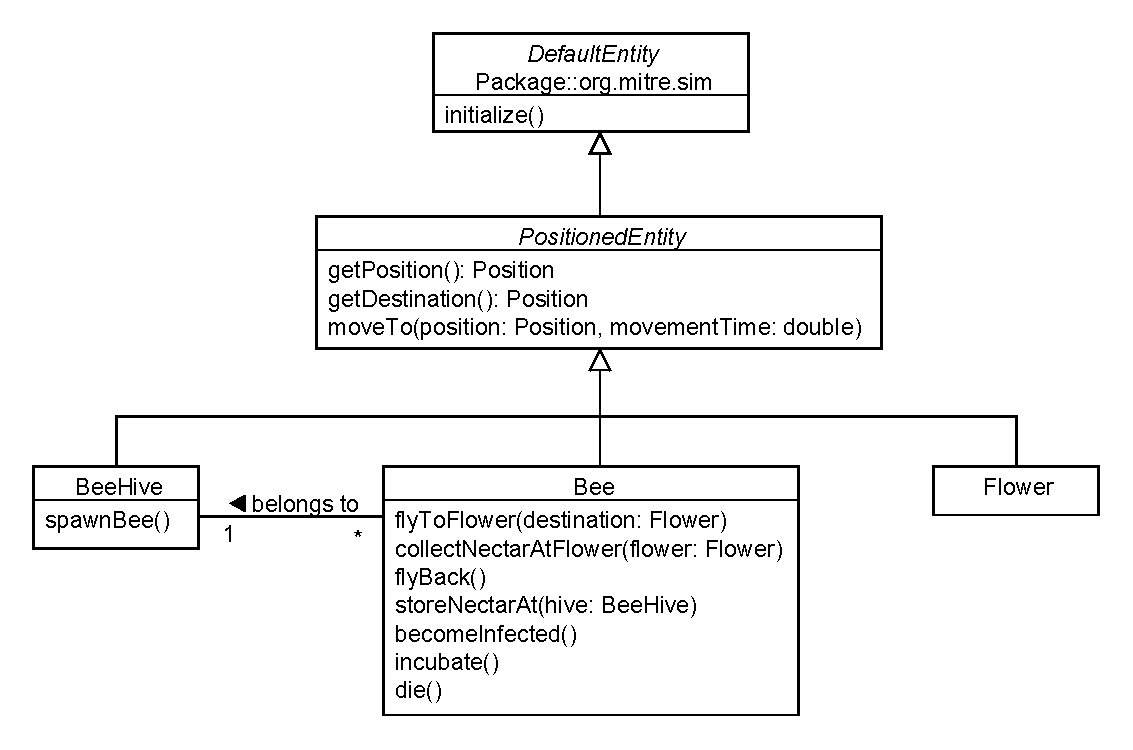
\includegraphics[width=1\linewidth]{entities}
  \caption{UML-Klassendiagramm der Simulationsentit�ten. Private oder nicht simulationsbezogene Methoden und Attribute wurden aus �bersichtlichkeitsgr�nden weggelassen.}
  \label{img:entities} 
	\end{center}
\end{figure}